\documentclass{article}
\usepackage[polish]{babel}
\usepackage[OT4]{fontenc}
\usepackage[utf8]{inputenc}
\usepackage{hyperref}
\usepackage{graphicx}
\usepackage{float}
\usepackage{amsmath}
\usepackage{indentfirst}
\usepackage{pythonhighlight}
\title{\textbf{Praca projektowa z przedmiotu Sztuczna Inteligencja}}
\author{Bartłomiej Czajka 169522 2 EF-DI P1}
\date{Rzeszów, 2023}
\linespread{1.5}
\begin{document}
\maketitle
\pagebreak



\tableofcontents{}
\section{Opis projektu}
\subsection{Założenia projektowe}
Celem projektu jest realizacja sieci neuronowej uczonej za pomocą algorytmu sieci głębokiej, klasyfikującej chorobę Parkinsona oraz zbadanie wpływu parametrów sieci na proces uczenia.
Projekt został zrealizowany w języku Python z wykorzystaniem biblioteki PyTorch.
\subsection{Zestaw danych}
Zestaw danych uczących został pobrany ze strony \href{http://archive.ics.uci.edu/ml/datasets/Parkinsons}{http://archive.ics.uci.edu/ml/datasets/Parkinsons}.
Zawiera on 197 instancji, 23 cechy oraz 2 klasy. Dane są nieuporządkowane, nie ma danych nieokreślonych.
Dokładniejszy opis cech zestawu:
\begin{itemize}
    \item name - Nazwa badanego pacjenta w ASCII i numer nagrania.
    \item MDVP:Fo(Hz) - Średnia częstotliwość podstawowa głosu.
    \item MDVP:Fhi(Hz) - Maksymalna częstotliwość podstawowa głosu.
    \item MDVP:Flo(Hz) - Minimalna częstotliwość podstawowa głosu.
    \item MDVP:Jitter(\%), MDVP:Jitter(Abs), MDVP:RAP, MDVP:PPQ, Jitter:DDP - Kilka miar zmienności częstotliwości podstawowej.
    \item MDVP:Shimmer, MDVP:Shimmer(dB), Shimmer:APQ3, Shimmer:APQ5, MDVP:APQ, Shimmer:DDA - Kilka miar zmienności amplitudy.
    \item NHR, HNR - Dwie miary stosunku szumu do składowych tonalnych w głosie.
    \item status - Stan zdrowia badanego (jeden) - chory na Parkinsona, (zero) - zdrowy.
    \item RPDE, D2 - Dwie miary złożoności dynamicznej nieliniowej.
    \item DFA - Wykładnik skalowania fraktalnego sygnału.
    \item spread1, spread2, PPE - Trzy nieliniowe miary zmienności częstotliwości podstawowej.
\end{itemize}
\subsection{Przygotowanie danych}
Sieć ma za zadanie sklasyfikować czy pacjent cierpi na chorobę Parkinsona. Wartość '1' oznacza osobę cierpiącą na chorobę Parkinsona, natomiast '0' oznacza osobę zdrową.
Dane zostały uporządkowane i znormalizowane.
Normalizacja została wykonana dla każdej obserwacji przy użyciu wzoru:
\[
    x_{\text{norm}} = \frac{{x_{\text{norm\_max}} - x_{\text{norm\_min}}}}{{x_{\text{max}} - x_{\text{min}}}} \cdot (x - x_{\text{min}}) + x_{\text{norm\_min}}
\]

gdzie:
\begin{itemize}
    \item $x_{min}$ - to wektor zawierający minimalne wartości dla każdej obserwacji.
    \item $x_{max}$ - to wektor zawierający maksymalne wartości dla każdej obserwacji.
    \item $x_{norm\_min}$ - to wartość minimalna po normalizacji (-1).
    \item $x_{norm\_max}$ - to wartość maksymalna po normalizacji (1).
    \item $x_{norm}$ - to macierz zawierająca znormalizowane dane.
    \item $x$ - to macierz zawierająca dane wejściowe.
\end{itemize}
\section{Zagadnienia teoretyczne}
\subsection{Matematyczny opis sztucznego neuronu}
Podstawowym elementem budującym strukturę sieci neuronowej jest neuron. Jest to element, który przetwarza informacje.
W pewnym, uproszczonym stopniu jest wzorowany na funkcjonowaniu biologicznej komórki nerwowej.
Struktura neuronu zawiera wiele wejść oraz jedno wyjście.
Jednym z najważniejszych składników neuronu są wagi, których wartości decydują o zachowaniu neuronu. Są one zazwyczaj ustalane w trakcie procesu uczenia.
\begin{figure}[H]
    \centering
    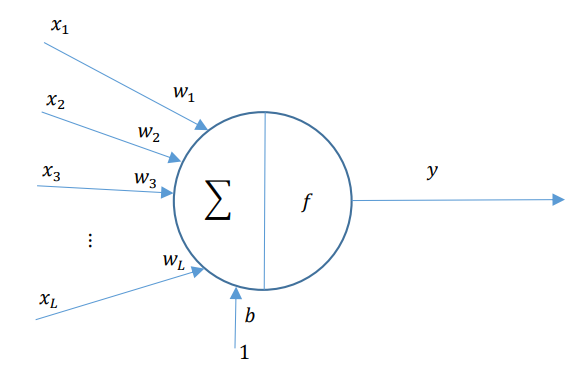
\includegraphics[width=0.8\textwidth, keepaspectratio]{model_neuronu.png}
    \caption{Model neuronu [4]}
    \label{fig:zdjecie}
\end{figure}

Każdy pojedynczy neuron przyjmuje sygnały wejściowe, które są następnie przetwarzane.
Każde wejście ma przypisany współczynnik wagowy, który określa jak bardzo wpływa ono na wynik neuronu.
Ponadto, neuron posiada "bias", czyli dodatkowe wejście, na którym występuje stała wartość.
Wszystkie te informacje są sumowane, aby obliczyć łączne pobudzenie neuronu.
Następnie wartość pobudzenia przechodzi przez funkcję aktywacji, która określa sygnał wyjściowy neuronu.

Wzór na łączne pobudzenie neuronu:
\[
    y = \sum_{j=1}^{L} f(w_{j} x_{j} + b)
\]

gdzie:
\begin{itemize}
    \item $j$ -- indeks, który przyjmuje wartości od 1 do $L$,
    \item $y$ -- wyjście neuronu,
    \item $w_{j}$ -- współczynnik wagowy przypisany do $j$-tego wejścia,
    \item $x_{j}$ -- $j$-ty sygnał wejściowy,
    \item $b$ -- bias [2].
\end{itemize}

\subsection{Funkcja aktywacji}
Sam model matematyczny neuronu nie byłby wystarczający do skomplikowanych obliczeń w m.in. sieciach głębokich.
Należy wprowadzić funkcje aktywacji, które nadają sieciom neuronowym zdolność modelowania nieliniowych relacji między danymi wejściowymi, a wyjściowymi.
Dzięki tej nieliniowej transformacji na wyjściu sztucznego neuronu, możliwe jest wprowadzenie nieliniowości i bardziej skomplikowanych obliczeń.

Istnieje wiele funkcji aktywacji.
Szczególnie przydatną w modelach głębokich ze względu na swoją prostotę i skuteczność jest funkcja ReLU, która została przeze mnie wykorzystana jako funkcja aktywacji dla warstw ukrytych.
Działa na zasadzie przekazywania wartości dodatnich bez ich zmiany, natomiast dla wartości ujemnych przypisuje zerową wartość.
Matematycznie można zdefiniować ją następującym wzorem:
\[
    f(x) = \max(0, x)
\]
Innymi słowy, funkcja ReLU jest zdefiniowana na przedziale:
\[
    f(x) = \begin{cases}
        0, & \text{gdy } x \leq 0, \\
        x, & \text{gdy } x > 0.
    \end{cases}
\]
gdzie:
\begin{itemize}
    \item $x$ -- wartość wejściowa, na której zostanie zastosowana funkcja aktywacji.
\end{itemize}

Istnieje również funkcja aktywacji softmax, która dla danego wektora wyników \( \mathbf{z} = (z_1, z_2, \ldots, z_n) \), gdzie \( n \) oznacza liczbę klas, przekształca każdy element \( z_i \) na wartość prawdopodobieństwa \( p_i \).
Funkcję softmax można zdefiniować w następujący sposób:
\[
    f(z)_i = \frac{e^{z_i}}{\sum_{j=1}^{n} e^{z_j}}
\]
gdzie:
\begin{itemize}
    \item \(f(z)_i\) -- \(i\)-ty element wyniku funkcji softmax dla wektora wyników \(\mathbf{z}\),
    \item \(e^{z_i}\) -- funkcja wykładniczą podniesiona do potęgi \(z_i\),
    \item \(z_i\) -- \(i\)-ty element wektora wyników,
    \item \(\sum_{j=1}^{n} e^{z_j}\) -- suma funkcji wykładniczych dla wszystkich elementów wektora wyników,
    \item \(n\) -- liczba klas.
\end{itemize}
Ostatnią funkcją aktywacji, którą wykorzystałem, jest funkcja sigmoidalna.
Analogicznie do funkcji softmax, została użyta do aktywacji warstwy wyjściowej.
Funkcja sigmoidalna przekształca wartość wejściową na wartość z zakresu (0, 1), co czyni ją przydatną w problemach klasyfikacji binarnej.
Matematycznie funkcję sigmoidalną można zdefiniować jako:
\[
    f(x) = \frac{1}{1 + e^{-x}}
\]
gdzie:
\begin{itemize}
    \item \(x\) -- wartość wejściowa do funkcji sigmoidalnej,
    \item \(e\) --  podstawa logarytmu naturalnego, przybliżone do wartości 2.71828,
    \item \(f(x)\) -- to wartość wyjściowa funkcji sigmoidalnej, przekształcająca \(x\) na wartość z przedziału (0, 1).
\end{itemize}
\subsection{Sieć głęboka}
Sieci głębokie to rodzaj modeli uczenia maszynowego, które składają się z wielu warstw neuronów, zwanych warstwami głębokimi.
Uczenie sieci głębokich opiera się na zasadzie propagacji wstecznej, która jest jednym z kluczowych algorytmów używanych do dostosowania wag sieci neuronowej w procesie uczenia.
Propagacja wsteczna umożliwia obliczenie gradientów wag sieci na podstawie funkcji kosztu i propaguje te gradienty wstecz przez sieć, aby zaktualizować wagi w celu minimalizacji błędu.
\begin{figure}[H]
    \centering
    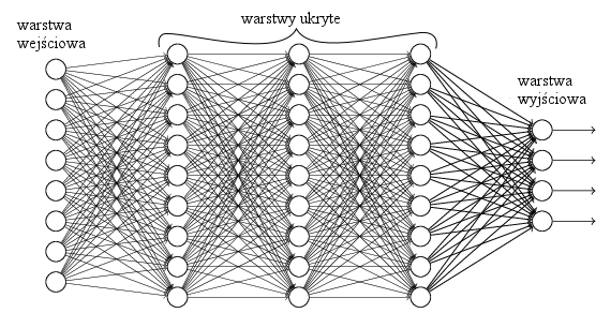
\includegraphics[width=1\textwidth, keepaspectratio]{siec_gleboka.png}
    \caption{Sieć głęboka [5]}
    \label{fig:siec}
\end{figure}


Proces uczenia sieci głębokich rozpoczyna się od inicjalizacji wag, które mogą być inicjalizowane losowo lub przy użyciu innych metod.
Następnie dane wejściowe są przekazywane od warstwy wejściowej do warstwy wyjściowej (ang. forward propagation).
Każda warstwa na podstawie wag i funkcji aktywacji oblicza swoje wyjście.
Na podstawie wyników obliczana jest wartość funkcji kosztu, która mierzy błąd przewidywań sieci.
Kolejnym krokiem jest wykorzystanie algorytmu propagacji wstecznej, który oblicza gradienty wag sieci neuronowej.
Gradienty oblicza się iteracyjnie, zaczynając od warstwy wyjściowej przechodząc wstecz przez kolejne warstwy sieci.
W dalszej kolejności, biorąc pod uwagę obliczone gradienty wag, wagi sieci są aktualizowane w celu zminimalizowania funkcji kosztu mierzącej błąd predykcji sieci.
Dokonuje się tego za pomocą optymalizatora (np. ADAM).
Wyżej wymienione kroki powtarza się aż do osiągnięcia zdefiniowanej liczby epok lub innych kryteriów zatrzymania.
\subsection{Funkcja kosztu}
Wykorzystaną funkcją kosztu w programie jest entropia krzyżowa.
Funkcja ta mierzy stopień niezgodności między rzeczywistymi etykietami, a przewidywanymi prawdopodobieństwami dla każdej klasy.
Im większa niezgodność, tym większa wartość funkcji kosztu.
Dąży się do minimalizacji tej funkcji, poprzez zmianę wag sieci.

Entropię krzyżową, w szczególności dla klasyfikacji binarnej, można zdefiniować następującym wzorem:
\begin{align*}
    H(y, p) & = -\sum_{i=1}^{C} y_i \log(p_i) =    \\
            & = -\sum_{i=1}^{2} y_i \log(p_i) =    \\
            & = -[y_1 \log(p_1) + y_2 \log(p_2)] = \\
            & = - [y \log(p) + (1-y) \log(1-p)]
\end{align*}

gdzie:
\begin{itemize}
    \item  \(H(y, p)\) -- wartość entropii krzyżowej,
    \item  \(y_i\) -- \(i\)-ta rzeczywista etykieta (0 lub 1) dla próbki i,
    \item  \(p_i\) -- \(i\)-te przewidziane prawdopodobieństwo dla próbki i,
    \item \(C\) -- liczba klas.
\end{itemize}

\subsection{Algorytm wstecznej propagacji błędu}
Algorytm wstecznej propagacji błędu, nazywany również algorytmem największego spadku gradientu, jest jednym z głównych algorytmów stosowanych w procesie uczenia sieci głębokich.
Umożliwia on aktualizację wag sieci w celu minimalizacji funkcji kosztu poprzez iterację przez kolejne warstwy sieci.
Proces ten można podzielić na dwa kroki: propagację w przód oraz wstecz.

Propagacja w przód polega na przekazywaniu danych wejściowych przez sieć od warstwy wejściowej do warstwy wyjściowej.
W każdej warstwie obliczane są aktywacje neuronów na podstawie obecnych wag i danych wejściowych.
Wyniki z danej warstwy przekazywane są do kolejnej aż do warstwy wyjściowej gdzie generowany jest wynik predykcji.

W propagacji wstecznej natomiast porównuje się wynik sieci z oczekiwanym wynikiem, obliczając przy tym błąd.
Błąd ten jest następnie propagowany wstecz od zaczynając od warstwy wyjściowej.
Obliczany jest gradient funkcji kosztu względem wag sieci, który informuje o kierunku dostosowania wag w celu minimalizacji błędu.
Na podstawie gradientu aktualizowane są wagi sieci przy użyciu odpowiedniej metody optymalizacji, takiej jak metoda spadku gradientu czy też jej wariant, np. ADAM.

\subsection{Metoda optymalizacji ADAM}
Metoda ADAM jest popularna w optymalizacji sieci głębokich, ponieważ łączy zalety adaptacyjnego skalowania kroku uczenia (RMSProp) i momentu, co prowadzi do efektywniejszej optymalizacji i szybszego zbiegania do optymalnych wag sieci.

Aby obliczyć gradient funkcji kosztu, należy obliczyć pochodne cząstkowe dla każdej warstwy, od ostatniej warstwy do pierwszej.
W każdej warstwie oblicza się lokalny gradient na podstawie pochodnej funkcji kosztu oraz gradientu z poprzedniej warstwy.

Wzór na gradient funkcji kosztu H, w kroku t:
\[ g_t = \frac{\partial H}{\partial W} \]
gdzie:
\begin{itemize}
    \item \( H\) -- funkcja kosztu,
    \item \(W\) -- macierz wag sieci neuronowej.
\end{itemize}

Algorytm ADAM składa się z następujących kroków:
\begin{enumerate}
    \item Obliczenie gradientów funkcji kosztu względem wag sieci za pomocą propagacji wstecznej błędu.
    \item Aktualizacja momentu gradientu \(m_t\) i drugiego momentu gradientu \(v_t\) na podstawie obliczonych gradientów.
    \item Obliczenie wygładzonych estymacji momentu i drugiego momentu: \(\hat{m}_t\) i \(\hat{v}_t\).
    \item Aktualizacja wag sieci z wykorzystaniem estymacji momentu i drugiego momentu, współczynnika uczenia \(\alpha\) oraz małej wartości epsilon \(\epsilon\).
\end{enumerate}

Gradient jest używany do aktualizacji wag zgodnie z następującymi wzorami:
\[m_t = \beta_1 \cdot m_{t-1} + (1 - \beta_1) \cdot g_t\]
\[v_t = \beta_2 \cdot v_{t-1} + (1 - \beta_2) \cdot g_t^2\]
\[\hat{m}_t = \frac{m_t}{1 - \beta_1^t}\]
\[\hat{v}_t = \frac{v_t}{1 - \beta_2^t}\]
\[ W_{t+1} = W_t - \frac{\eta}{\sqrt{\hat{v}_t} + \epsilon} \cdot \hat{m}_t \]
gdzie:
\begin{itemize}
    \item \(m_t\) to estymacja momentu gradientu w kroku czasowym \(t\).
    \item \(v_t\) to estymacja drugiego momentu gradientu w kroku czasowym \(t\).
    \item \(\beta_1\) i \(\beta_2\) to współczynniki z zakresu \([0, 1)\) kontrolujące eksponencjalne wygładzanie momentu i drugiego momentu.
    \item \(\alpha\) to współczynnik uczenia (learning rate).
    \item \(\epsilon\) to mała wartość (np. \(10^{-8}\)) używana w celu uniknięcia dzielenia przez zero.
    \item \(\hat{m}_t\) i \(\hat{v}_t\) to wygładzone estymacje momentu i drugiego momentu.
    \item \(W_{t}\) i \(W_{t+1}\) to wagi w krokach czasowych \(t\) i \(t+1\).
\end{itemize}
Przy użyciu tych wzorów, w metodzie optymalizacji ADAM aktualizuje się wagi sieci neuronowej, wykorzystując estymację momentu i drugiego momentu gradientu.
To pozwala na efektywną optymalizację sieci głębokiej, dostosowując krok uczenia (learning rate) dla każdej wagi indywidualnie.
\section{Realizacja sieci neuronowej}
\subsection{Opis skryptu}
Skrypt został podzielony na kilka innych.
Każdy ze skryptów dotyczy poprawności klasyfikacji w zależności od różnych parametrów.
W każdym ze skryptów występuje ta sama początkowa część, która zawiera przetwarzanie danych zawartych w pliku "parkinsons.txt", normalizuje je, sortuje i zapisuje przetworzone dane do pliku "parkinsons.hkl".
Następnie dane wejściowe są skalonwane i dzielone na zbiór treningowy i testowy.
Wektory "y" są przekształcane tak, aby indeks pierwszej klasy wynosił 0.
Dalsza część skryptu różni się dla poszczególnych wersji.
\subsection{Początek każdego ze skryptów}
\begin{python}
    from torch.autograd import Variable
    import torch.nn as nn
    import torch.nn.functional as F
    import torch
    import numpy as np
    import matplotlib.pyplot as plt
    import hickle as hkl
    from sklearn.model_selection import train_test_split
    from sklearn.preprocessing import StandardScaler

    """Data preparation with manual deletion of the first line (feature names)"""
    filename = "parkinsons.txt"
    data = np.loadtxt(filename, delimiter=",", dtype=str)
    x = np.concatenate((data[:, 1:17], data[:, 18:]), axis=1).astype(float).T
    y_t = data[:, 17].astype(float)
    y_t = y_t.reshape(1, y_t.shape[0])
    np.transpose([np.array(range(x.shape[0])), x.min(axis=1), x.max(axis=1)])

    # Normalization
    x_min = x.min(axis=1)
    x_max = x.max(axis=1)
    x_norm_max = 1
    x_norm_min = -1
    x_norm = np.zeros(x.shape)
    for i in range(x.shape[0]):
    x_norm[i, :] = (x_norm_max - x_norm_min) / (x_max[i] - x_min[i]) * (
    x[i, :] - x_min[i]
    ) + x_norm_min
    np.transpose([np.array(range(x.shape[0])),
            x_norm.min(axis=1), x_norm.max(axis=1)])

    # Before sorting
    plt.plot(y_t[0])
    plt.show()

    y_t_s_ind = np.argsort(y_t)
    x_n_s = np.zeros(x.shape)
    y_t_s = np.zeros(y_t.shape)
    for i in range(x.shape[1]):
    y_t_s[0, i] = y_t[0, y_t_s_ind[0, i]]
    x_n_s[:, i] = x_norm[:, y_t_s_ind[0, i]]

    # After sorting
    plt.plot(y_t_s[0])
    plt.show()

    hkl.dump([x, y_t, x_norm, x_n_s, y_t_s], "parkinsons.hkl")
    x, y_t, x_norm, x_n_s, y_t_s = hkl.load("parkinsons.hkl")
    if min(y_t.T)[0] > 0:
    y = y_t.squeeze() - 1  # index of first class should equal to 0
    else:
    y = y_t.squeeze()
    X = x.T

    # Scale data to have mean 0 and variance 1
    # which is importance for convergence of the neural network
    scaler = StandardScaler()
    X_scaled = scaler.fit_transform(X)

    # Split the data set into training and testing
    X_train, X_test, y_train, y_test = train_test_split(
    X_scaled, y, test_size=0.2, random_state=2
    )
\end{python}
\subsection{Skrypt dla zależności poprawności klasyfikacji od liczby neuronów w warstwach}
\begin{python}
    class Model(nn.Module):
    def __init__(self, input_dim, output_dim, K1, K2):
    super(Model, self).__init__()
    self.layer1 = nn.Linear(input_dim, K1)
    self.layer2 = nn.Linear(K1, K2)
    self.layer3 = nn.Linear(K2, output_dim)

    def forward(self, x):
    x = F.relu(self.layer1(x))
    x = F.relu(self.layer2(x))
    x = F.softmax(self.layer3(x), dim=1)
    return x


    lr_vec = np.array([1e-1, 1e-2, 1e-3, 1e-4, 1e-5, 1e-6, 1e-7])
    K1_vec = np.arange(40, 1000, 30)
    K2_vec = K1_vec
    PK_2D_K1K2 = np.zeros([len(K1_vec), len(K2_vec)])
    max_epoch = 4000
    PK_2D_K1K2_max = 0
    k1_ind_max = 0
    k2_ind_max = 0
    X_train = Variable(torch.from_numpy(X_train)).float()
    y_train = Variable(torch.from_numpy(y_train)).long()
    X_test = Variable(torch.from_numpy(X_test)).float()
    y_test = Variable(torch.from_numpy(y_test)).long()
    for k1_ind in range(len(K1_vec)):
    for k2_ind in range(len(K2_vec)):
    model = Model(X_train.shape[1], int(
    max(y) + 1), K1_vec[k1_ind], K2_vec[k2_ind])
    optimizer = torch.optim.Adam(model.parameters(), lr=lr_vec[0])
    loss_fn = nn.CrossEntropyLoss()

    for epoch in range(max_epoch):
    y_pred = model(X_train)
    loss = loss_fn(y_pred, y_train)

    optimizer.zero_grad()
    loss.backward()
    optimizer.step()

    with torch.no_grad():
    y_pred = model(X_test)
    correct = (torch.argmax(y_pred, dim=1) ==
    y_test).type(torch.FloatTensor)
    PK = correct.mean().item() * 100
    print("K1 {} | K2 {} | PK {} ".format(
    K1_vec[k1_ind], K2_vec[k2_ind], PK))
    PK_2D_K1K2[k1_ind, k2_ind] = PK

    if PK > PK_2D_K1K2_max:
    PK_2D_K1K2_max = PK
    k1_ind_max = k1_ind
    k2_ind_max = k2_ind

    fig = plt.figure(figsize=(8, 8))
    ax = fig.add_subplot(111, projection="3d")
    X, Y = np.meshgrid(K1_vec, K2_vec)
    surf = ax.plot_surface(X, Y, PK_2D_K1K2.T, cmap="viridis")
    ax.set_xlabel("K1")
    ax.set_ylabel("K2")
    ax.set_zlabel("PK")
    ax.view_init(30, 200)
    plt.savefig("Fig.1_PK_K1K2_pytorch_parkinsons.png", bbox_inches="tight")

\end{python}
Na początku skryptu zostaje zdefiniowana klasa Model, która dziedziczy po module "nn.Module".
Jest to model sieci neuronowej.
W konstruktorze zdefiniowana zostaje struktura modelu, tj. warstwy liniowe (nn.Linear) i ich rozmiary.
W klasie zostaje zdefiniowana metoda "forward", która definiuje przepływ danych przez model.
Metoda wykorzystuje funkcje aktywacji ReLU oraz funkcję softmax na ostatniej warstwie.
Kolejną częscią kodu jest definicja parametrów uczenia.
Oto ich opis:
\begin{itemize}
    \item \texttt{lr\_vec} -- wektor współczynników uczenia, czyli prędkości z jaką model aktualizuje wagi w czasie uczenia,
    \item \texttt{K1\_vec} oraz \texttt{K2\_vec} -- wektory, które odpowiadają rozmiarom warstw w modelu. Generowane są przy wykorzystaniu \texttt{np.arange},
    \item \texttt{PK\_2D\_K1K2} -- macierz, która będzie przechowywać wyniki ocenu modelu dla różnych kombinacji,
    \item \texttt{max\_epoch} -- oznacza maksymalną liczbę epok,
    \item \texttt{PK\_2D\_K1K2\_max} -- dotychczasowa maksymalna poprawność klasyfikacji,
    \item \texttt{k1\_ind\_max}, \texttt{k2\_ind\_max} -- indeksy kombinacji rozmiarów warstw odpowiednio \texttt{K1} oraz \texttt{K2}, dla których uzyskano najwyższą ocenę \texttt{PK\_2D\_K1K2\_max},
    \item \texttt{X\_train}, \texttt{y\_train} -- dane treningowe,
    \item \texttt{X\_test}, \texttt{y\_test} -- dane testowe.
\end{itemize}
Zagnieżdżone pętle `for' iterują po rozmiarach `K1' oraz `K2'. Tworzony jest model z odpowiednimi rozmiarami warstw i definiowany jest optymalizator (ADAM) oraz funkcja kosztu.
W pętli treningowej obliczane są predykcje modelu, strata oraz aktualizowane są wagi modelu.
Po zakończeniu treningu, obliczana jest ocena `PK' dla danych testowych.
Jeżeli aktualna poprawność klasyfikacji jest większa od dotychczasowej, maksymalnej, aktualizowane są odpowiednie zmienne.
Na końcu skryptu, tworzony jest wykres 3D, w którym oś X reprezentuje `K1', oś Y reprezentuje `K2' natomiast oś Z reprezentuje poprawność klasyfikacji (PK).
Wykres jest zapisywany jako obraz z rozszerzeniem PNG.


\section{Eksperymenty}
Dla każdego eksperymentu został użyty inny skrypt.
Pierwsze eksperymenty będą dotyczyć rozmiaru warstw, natomiast kolejne zmian współczynniku uczenia, liczby warstw oraz funkcji przejścia.
\subsection{Eksperyment 1}
Eksperyment pierwszy został przeprowadzony dla przykładowych liczb neuronów będących wielokrotnościami liczby 2.
Warstwa pierwsza zawiera liczbę neuronów z zakresu ZAKRES, natomiast warstwa druga z zakresu ZAKRES.
Współczynnik uczenia wynosi $0.1$, natomiast liczba epok $100$.
\subsection{Eksperyment 2}
\subsection{Eksperyment 3}
\section{Wnioski}
\begin{thebibliography}{9}
    \bibitem{Nielsen}
    Michael Nielsen,
    \emph{Neural Networks and Deep Learning}.
    Determination Press,
    2015.
    \bibitem{TadeusiewiczSzaleniec}
    Ryszard Tadeusiewicz, Maciej Szaleniec,
    \emph{Leksykon sieci neuronowych}.
    Wrocław,
    2015.
    \bibitem{vandeput}
    Nicolas Vandeput,
    \href{https://medium.com/analytics-vidhya/a-brief-history-of-neural-networks-c234639a43f1}{\emph{A Brief History Of Neural Networks}},
    [dostęp: 17.05.2023].
    \bibitem{zajdel}
    Zajdel R.,
    \emph{Ćwiczenie 4 Model Neuronu},
    Rzeszów,
    KIiA, PRz.
    \bibitem{gora}
    Paweł Gora,
    \href{https://www.deltami.edu.pl/temat/informatyka/sztuczna_inteligencja/2017/12/28/Glebokie_uczenie_maszyn/}{\emph{Głębokie uczenie maszyn}},
    [dostęp: 17.05.2023].
    \bibitem{zajdel}
    Zajdel R.,
    \emph{Procedura przygotowania danych dla sieci neuronowych na potrzeby projektu z modułu sztuczna inteligencja - Listing1},
    Rzeszów,
    KIiA, PRz.
    \bibitem{zajdel}
    Zajdel R.,
    \emph{Procedura przygotowania danych dla sieci neuronowych na potrzeby projektu z modułu sztuczna inteligencja - Listing2},
    Rzeszów,
    KIiA, PRz.
\end{thebibliography}
\end{document}